\section{Undecided State Dynamics}
\label{undecided}

In this transition rule, the randomly selected agent observes the opinion of another randomly selected agent. If the selected agent encounters a differing opinion, he becomes “undecided”. Undecided agents adopt any decided opinions that they encounter.

\begin{figure}[H]
     \centering
     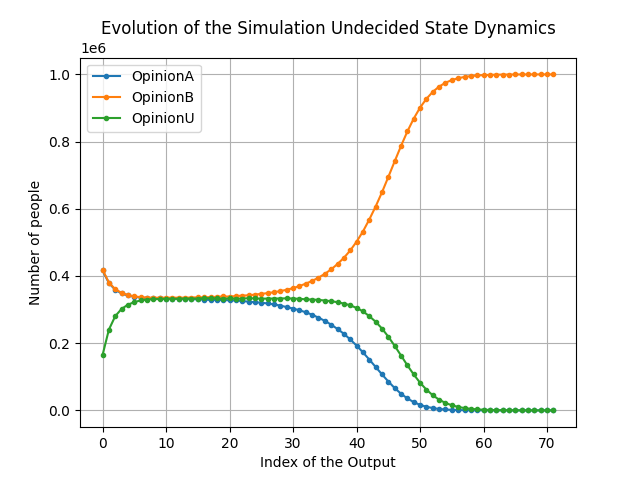
\includegraphics[width=0.78\textwidth,height=0.32\textheight]{img/svg/Undecided/1mln/withoutTime.png}
     \caption{Simulation done with 1mln agents, output each 500 000 iteration}
\end{figure}
\begin{figure}[H]
     \centering
     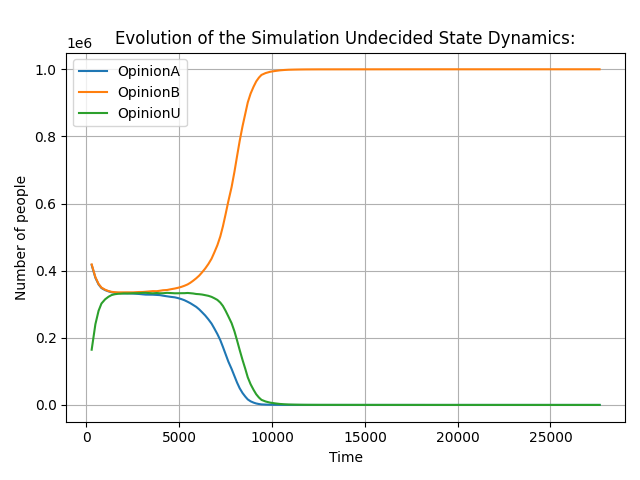
\includegraphics[width=0.75\textwidth,height=0.32\textheight]{img/svg/Undecided/1mln/withTime.png}
     \caption{Simulation done with 1mln of agents, Time calculated in ms}
\end{figure}

\begin{figure}[H]
     \centering
     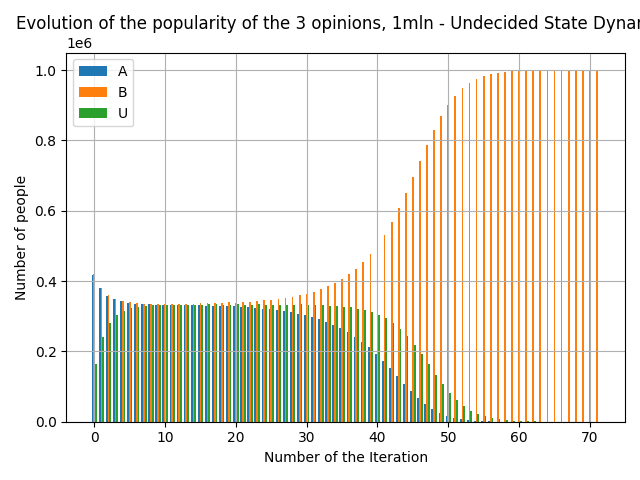
\includegraphics[width=0.80\textwidth,height=0.37\textheight]{img/svg/Undecided/1mln/barChart.png}
     \caption{Simulation done with 1mln of agents}
\end{figure}



In these graphs, we can see, that at first the number of decided opinions falls, while the number of undecided opinions rises, this goes on until some of the one of decided opinions starts gaining numbers, while the other types rapidly fall. This makes sense because at the start we have an even amount of agents with opinion A and opinion B. The probability that an agent observes an agent of a differing opinion is pretty much 0.5 and then the agent becomes undecided. \\

The plots below show the behavior of the algorithm with 10mln and 100mln of agents. As we can see the evolution of the line is approximately the same as with 1mln agents, for this reason there isn’t much to say about them.

\begin{figure}[!ht]
     \includegraphics[width=0.40\textwidth,height=0.15\textheight]{img/svg/Undecided/10mln/withoutTime.png}
     \centering
     \includegraphics[width=0.40\textwidth,height=0.15\textheight]{img/svg/Undecided/10mln/withTime.png}
     \caption{Simulation done with 10mln agents, Time in ms}
\end{figure}
\begin{figure}[!ht]
     \includegraphics[width=0.40\textwidth,height=0.15\textheight]{img/svg/Undecided/100mln/withoutTime.png}
     \centering
     \includegraphics[width=0.40\textwidth,height=0.15\textheight]{img/svg/Undecided/100mln/withTime.png}
     \caption{Simulation done with 100mln agents, Time in ms}
\end{figure}

In the following plot there is an interesting find, the time difference in running time is a lot smaller between 10 and a 100 million agents, than the time between 1 and 10 million agents. The difference between 1 million agents and 10 million agents is more than 20x, but the difference between 10 million agents and 100 million agents is less than 2x.

\begin{figure}[H]
     \centering
     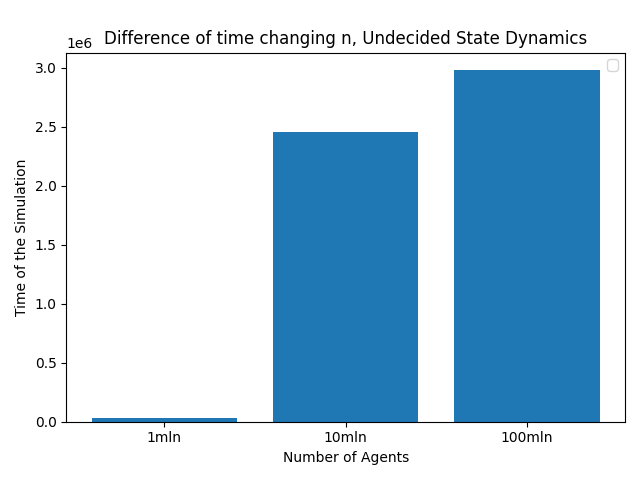
\includegraphics[width=0.80\textwidth,height=0.37\textheight]{img/svg/Undecided/TimeDifferenceN.png}
\end{figure}
\newpage

\subsection[0.5-0.75 Undecided State Dynamics]{Comparison between 0.5 and 0.75, Undecided State Dynamics simulation}

Just like the other two models, the change of number of iterations and time was negative for the Undecided State Model as well. The time taken decreased from 2.5 ms to 800,000 ms. And the number of iterations decreased from 350,000,000 iterations to around 150,000,000 iterations.

\begin{figure}[H]
     \centering
     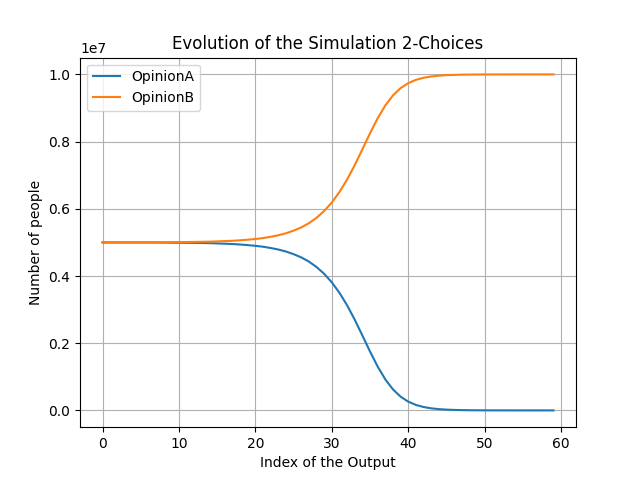
\includegraphics[width=0.60\textwidth,height=0.23\textheight]{img/svg/0.75/Undecided/withoutTime.png}
     \caption{Probability A 0.75, output each 5 million iteration}
\end{figure}
\begin{figure}[H]
     \centering
     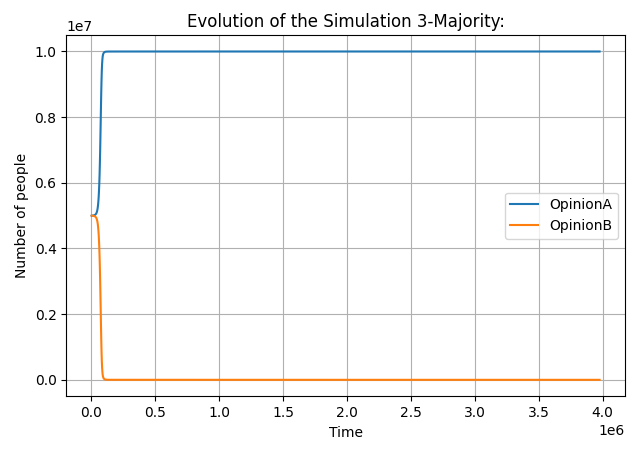
\includegraphics[width=0.60\textwidth,height=0.23\textheight]{img/svg/0.75/Undecided/withTime.png}
     \caption{Probability A 0.75, Time calculated in ms}
\end{figure}
\begin{figure}[H]
     \centering
     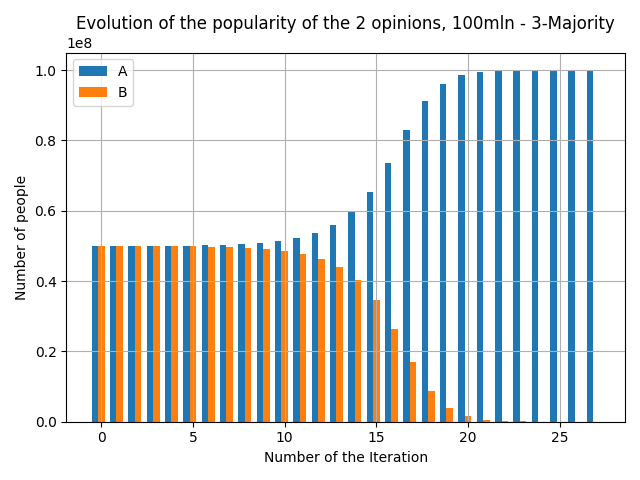
\includegraphics[width=0.60\textwidth,height=0.23\textheight]{img/svg/0.75/Undecided/barChart.png}
     \caption{Probability A 0.75, Done with 10mln of agents}
\end{figure}